\documentclass[preprint]{sigplanconf}
\pdfpagewidth=8.5in 
\pdfpageheight=11in 

\usepackage{amsmath,amsthm,amssymb,epsfig,wrapfig,url,verbatim, fancyvrb,
            color,multirow}
            
\usepackage{float}


\newcommand{\rom}[1]{\uppercase\expandafter{\romannumeral #1\relax}}


\usepackage{lmodern}
\usepackage[utf8]{inputenc} 
\usepackage[T1]{fontenc}
\usepackage{microtype} 

%\usepackage[numbers]{natbib}

\usepackage[caption=false,font=scriptsize]{subfig}

\usepackage[normalem]{ulem}
\usepackage{hyperref}
\usepackage{paralist}



\usepackage{courier}            % standard fixed width font
\usepackage[scaled]{helvet} % see www.ctan.org/get/macros/latex/required/psnfss/psnfss2e.pdf

\usepackage{listings}          % format code
\usepackage{enumitem}      % adjust spacing in enums


% known bug: http://tex.stackexchange.com/questions/1522/pdfendlink-ended-up-in-different-nesting-level-than-pdfstartlink
%\newcommand{\doi}[1]{doi:~\href{http://dx.doi.org/#1}{\Hurl{#1}}}   % print a hyperlinked DOI
% http://dx.doi.org/10.1145/2737924.2738001

\setcounter{secnumdepth}{3}

\newtheorem{define}{Definition}[section]
\newtheorem{prop}{Property}[section]
\newtheorem{assume}{Assumption}
\newtheorem{theorem}{Theorem}
\newtheorem{lemma}{Lemma}[section]


\usepackage{balance}
%\usepackage{setspace}

\usepackage{booktabs}


%\usepackage{amsthm}

%\newtheoremstyle{exampstyle}
%  {\topsep} % Space above
%  {\topsep} % Space below
%  {} % Body font
%  {} % Indent amount
%  {\bfseries} % Theorem head font
%  {.} % Punctuation after theorem head
%  {.5em} % Space after theorem head
%  {} % Theorem head spec (can be left empty, meaning `normal')




\newcommand{\erf}[1]{Equation~(\ref{eq:#1})}
\newcommand{\erfs}[2]{Equations~(\ref{eq:#1} and~\ref{eq:#2})}
\newcommand{\srf}[1]{Section~\ref{sec:#1}}
\newcommand{\srfs}[2]{Sections~\ref{sec:#1} and~\ref{sec:#2}}
\newcommand{\frf}[1]{Figure~\ref{fig:#1}}
\newcommand{\frfs}[2]{Figures~\ref{fig:#1} and~\ref{fig:#2}}
\newcommand{\trf}[1]{Table~\ref{tab:#1}}
\newcommand{\trfs}[2]{Tables~\ref{tab:#1} and~\ref{tab:#2}}
\newcommand{\thm}[1]{Theorem~\ref{th:#1}}
\newcommand{\thms}[2]{Theorems~\ref{th:#1} and~\ref{th:#2}}
\newcommand{\step}[1]{Step~\ref{step:#1}}


\newcommand{\tabincell}[2]{\begin{tabular}{@{}#1@{}}#2\end{tabular}}

\newcommand{\naive}{na\"\i{}ve}
\newcommand{\Naive}{Na\"\i{}ve}

\newcommand{\TODO}[1]{\textbf{[TODO: #1]}}

\newcommand{\name}{{\sf Light}\xspace}
%\textsc{grail}

\hyphenation{light-weight}
\hyphenation{open-ldap}
\hyphenation{atomicity}

\newcounter{MYenumctr}
\newenvironment{MYenum}{\begin{list}{\arabic{MYenumctr}.}{%
\usecounter{MYenumctr}%
\setlength{\topsep}{0pt plus 0pt minus 0pt}%
\setlength{\itemsep}{0pt plus 0pt minus 0pt}%
\setlength{\parsep}{0pt plus 0pt minus 0pt}%
\setlength{\parskip}{0pt plus 0pt minus 0pt}%
}}{\end{list}}

\setlength{\abovecaptionskip}{3pt plus 0pt minus 0pt}
\setlength{\belowcaptionskip}{-15pt plus 2pt minus 2pt}
%\setlength{\intextsep}{10pt plus 2pt minus 2pt}
\usepackage[ruled,linesnumbered]{algorithm2e}
\renewcommand{\algorithmcfname}{ALGORITHM}


% to allow verbatim inside subfloat


\newcommand{\OmerEdit}[1]{{\color{red} #1}}

\newcommand{\Yunhui}[1]{{\color{blue} #1}}
\newcommand{\wrDepName}{flow-before\xspace}
\newcommand{\wrDep}{\lessdot}
\newcommand{\varAccessed}{\nu}
\newcommand{\getThread}{\tau}


\newcommand{\superscript}[1]{\ensuremath{^{\textrm{#1}}}}
\def\sharedaffiliation{\end{tabular}\newline\begin{tabular}{c}}


\makeatletter
\def \@ivtitleauthors#1#2#3#4{%
  \if \@andp{\@emptyargp{#2}}{\@emptyargp{#3}}%
    \noindent \@setauthor{40pc}{#1}{\@false}\par
  \else\if \@emptyargp{#3}%
    \noindent \@setauthor{17pc}{#1}{\@false}\hspace{3pc}%
              \@setauthor{17pc}{#2}{\@false}\par
  \else\if \@emptyargp{#4}%
    \noindent \@setauthor{17pc}{#1}{\@false}\hspace{3pc}%
              \@setauthor{17pc}{#3}{\@false}\par
  \else
    \noindent \@setauthor{9.3333pc}{#1}{\@false}\hspace{1.5pc}%
              \@setauthor{9.3333pc}{#2}{\@false}\hspace{1.5pc}%
              \@setauthor{9.3333pc}{#3}{\@false}\hspace{1.5pc}%
              \@setauthor{9.3333pc}{#4}{\@true}\par
    \relax
  \fi\fi\fi
  \vspace{20pt}}
\def \@maketitle {%
  \begin{center}
  \@settitlebanner
  \let \thanks = \titlenote
  {\leftskip = 0pt plus 0.25\linewidth
   \rightskip = 0pt plus 0.25 \linewidth
   \parfillskip = 0pt
   \spaceskip = .7em
   \noindent \LARGE \bfseries \@titletext \par}
  \vskip 6pt
  \noindent \Large \@subtitletext \par
  \vskip 12pt
  \ifcase \@authorcount
    \@latex@error{No authors were specified for this paper}{}\or
    \@titleauthors{i}{}{}\or
    \@titleauthors{i}{ii}{}\or
    \@titleauthors{i}{ii}{iii}\or
    \@ivtitleauthors{i}{ii}{iii}{iv}\or
    \@titleauthors{i}{ii}{iii}\@titleauthors{iv}{v}{}\or
    \@titleauthors{i}{ii}{iii}\@titleauthors{iv}{v}{vi}\or
    \@titleauthors{i}{ii}{iii}\@titleauthors{iv}{v}{vi}%
                  \@titleauthors{vii}{}{}\or
    \@titleauthors{i}{ii}{iii}\@titleauthors{iv}{v}{vi}%
                  \@titleauthors{vii}{viii}{}\or
    \@titleauthors{i}{ii}{iii}\@titleauthors{iv}{v}{vi}%
                  \@titleauthors{vii}{viii}{ix}\or
    \@titleauthors{i}{ii}{iii}\@titleauthors{iv}{v}{vi}%
                  \@titleauthors{vii}{viii}{ix}\@titleauthors{x}{}{}\or
    \@titleauthors{i}{ii}{iii}\@titleauthors{iv}{v}{vi}%
                  \@titleauthors{vii}{viii}{ix}\@titleauthors{x}{xi}{}\or
    \@titleauthors{i}{ii}{iii}\@titleauthors{iv}{v}{vi}%
                  \@titleauthors{vii}{viii}{ix}\@titleauthors{x}{xi}{xii}%
  \else
    \@latex@error{Cannot handle more than 12 authors}{}%
  \fi
  \vspace{1.75pc}
  \end{center}}
\makeatother




%\makeatletter
%\let\@copyrightspace\relax
%\makeatother


\begin{document}

\conferenceinfo{PLDI'15}{June 13--17, 2015, Portland, OR, USA}
\CopyrightYear{2015}
\crdata{978-1-4503-3468-6/15/06}

%http://dx.doi.org/10.1145/2737924.2738001



\title{Software Testing as a Compressed Sensing Problem}


\authorinfo{XXX}


\maketitle


\begin{abstract}
%\begin{abstract}
	Testing is perhaps the most popular way of ensuring software quality. Despite that, there are few principled methods to automatically test software, delta debugging being a notable exception. The gap that we address in this paper is how to efficiently test a software system under black-box assumptions with clearly articulated formal guarantees, where by efficiency we mean that only a small proportion of the overall test inputs is tried by the testing algorithm, and by formal guarantees we mean that the number of tests and probability of success follow from the testing framework.
	
	We address this challenge by making novel use of a technique from the area of signal processing known as \emph{compressed sensing}, and in particular its boolean variant known as \emph{group testing}. The key idea is to identify tests of interest by testing the system with random inputs that capture its input/output behavior, where group testing prescribes that tests are grouped together to minimize the number of inputs with a mathematical procedure how to recover single-element information from the results w.r.t. groups.
	
	As preliminary validation of the efficacy of compressed sensing in software testing, we report on experiments with web sanitizers and validators. The test inputs are cross-site scripting (XSS) payloads, and the output is a boolean indication whether or not the payloads penetrated through the built-in defenses. We demonstrate our ability to crack such defenses using only XXX tests, where brute-force testing would require XXX tests. This marks an XXX\% drop. 
\end{abstract}

\end{abstract}


%\category{D.2.5}{Software Engineering}{Testing and Debugging}

% general terms are not compulsory anymore, 
% you may leave them out
%\terms
%Design, Performance, Reliability

%\keywords
%Concurrency, Replay, Thread Determinism, Tight Bound, Local Recording







%\begin{theorem}[Correctness]\label{thm:correct}
%With the {\sf Grail} fix applied, the input bug does not manifest at runtime, and equally importantly, the fix does not cause new deadlocks to arise between any pair of threads.
%\end{theorem}
%
%\begin{proof}[Sketch]
%Deadlock freedom (over pairs of threads) is guaranteed by the fact that the Petri net models all relevant lock operations. Reasoning applied to the model detects, in addition to the buggy states pertaining to the input bugs, also the potential buggy (deadlock) states.
%\end{proof}



\section{Introduction}

\begin{enumerate}
	\item background / motivation
	\item existing approaches
	\item our approach
	\item contributions
\end{enumerate}

\section{The Theory Compressed Sensing}

\begin{enumerate}
	\item background (including main applications domains)
	\item main definitions, theorems and guarantees
\end{enumerate}
 
\section{Testing Algorithm}

\begin{enumerate}
	\item algorithm description (with pseudocode algorithm)
	\item walkthrough with explanations, etc
\end{enumerate}

\section{Formal Analysis and Guarantees}

\begin{enumerate}
	\item complexity
	\item precision / recall
	\item applicability
	\item etc
\end{enumerate}

\section{Implementation and Evaluation}
In this section, we describe a framework for applying group testing to the problem of explaining sanitizers. We begin with an explanation of the data generation, followed by a description of some simple sanitizers, and then explain how the framework is used to explain the sanitizers.

\subsection{Data Generation}
In general, any set we describe is based on an alphabet $\Sigma=\{x_1,\ldots,x_n\}$ comprised of $n$ tokens $x_i$ for $i=1,\ldots,n$. There are a finite number of strings that can be created based on the alphabet $\Sigma$ and we denote the set of possible strings as $\Sigma^*$. In any experiment, we will sample $m$ strings from $\Sigma^*$ and run a particular sanitizer on the $m$ strings to generate a vector $b$ that indicates whether or not each sample string is blocked by the sanitizer. Two questions remain: how to represent each string and how to sample each string. 

We discuss two string representations. Both representations define the matrix $A$ in the group testing formulation, where the $i^{th}$ row of $A$ represents the $i^{th}$ string. The first representation is token-based and was already described in Section \ref{ss:grouptesting_optimization}. In this representation, matrix $A$ has $n$ columns where $n$ is the number of individual tokens. The $i^{th}$ string is represented by $A_{i\cdot}$ where $A_{ij}=1$ if token $j$ appears in the string and $A_{ij}=0$ if it does not appear. The second representation is pattern-based and only keeps track of what possible patterns can appear in strings. We represent patterns as tuples of tokens such as (``$a$",``$b$",``$c$") for a pattern consisting of the three tokens ``$a$",``$b$",``$c$". Such a representation requires a priori knowledge about the grammar of a language and a fixed bank of possible patterns. Then the $i^{th}$ string is represented by $A_{i\cdot}$ where $A_{ij}=1$ if pattern $j$ appears in the string and $A_{ij}=0$ if it does not appear.

Our experiments consist of an alphabet consisting of 70 tokens:
$$
\begin{array}{ccc}
\sf{<} & \sf{script} & \sf{>} \\
\sf{\%PROBE\_STRING\%}  &   \sf{+} &  \sf{\{}   \\
\sf{toString} & \sf{:} & \sf{alert} \\
\sf{\}} & \sf{/} & \sf{\backslash n} \\
\sf{javascript:} &  \sf{\backslash t} & \sf{valueOf} \\
\sf{(} & \sf{)} & \sf{eval} \\
\sf{'} & \sf{ale} & \sf{rt} \\
\sf{/.source} & \sf{x=} & \\
\sf{;} & \sf{,} & \sf{input} \\
\sf{autofocus} & \sf{onfocus} & \sf{=} \\
\sf{`} & \sf{style} & \sf{div} \\
\sf{font-family} & \sf{expression} & \sf{span} \\
\sf{img} & \sf{a} & \sf{color} \\
\multicolumn{1}{c}{\sf{expres\backslash \backslash 73ion}} &
\multicolumn{1}{c}{\sf{expres\backslash \backslash 0073ion}} &
\multicolumn{1}{c}{\sf{expres\backslash \backslash 000073ion}} \\
\sf{@import} & \sf{http://} & \sf{.com} \\
\sf{https://} & \sf{:\backslash } & \sf{\backslash } \\
\sf{.org} & \sf{.net} & \sf{url(} \\
\sf{src} & \sf{x} & \sf{onerror} \\
\sf{http://ibm.com/x.jpg} & \sf{onmouseover} & \sf{http://ibm.com} \\
\sf{STUB} & \sf{\backslash \backslash } & \sf{b} \\
\sf{\backslash \backslash \backslash \backslash } & \sf{link} &  \sf{rel} \\
\sf{stylesheet} & \sf{type} & \sf{text/css} \\
\sf{href} & \sf{</} & \sf{/>} \\
\multicolumn{3}{c}{\sf{\backslash \backslash x61\backslash \backslash x6c\backslash \backslash x65\backslash \backslash x72\backslash \backslash x74\backslash \backslash x28\backslash \backslash x31\backslash \backslash x29}}
\end{array}
$$
These tokens are based on a data set used in \cite{TrippIssta:2013}.

We next address how to sample strings. In order to learn the tokens that truly explain a sanitizer (which we will refer to as the \emph{blocking tokens}), our sample of strings needs to satisfy the following conditions: 
\begin{itemize}
	\item We must observe the blocking tokens in \emph{enough} strings to be explainable. How much is \emph{enough} depends on how many observations of the token are needed to get K-disjunctness so that recovery is possible (see Theorem \ref{thm:LP_recovery}). 
	\RDTODO{FIX THIS STATEMENT}
	\item We must observe a sufficient number of blocked and unblocked strings. Specifically, we should observe 50\% blocked and 50\% unblocked strings. Intuitively, if we observe only blocked or only unblocked strings, it would be impossible to explain a sanitizer, so we must observe a mix. Mathematically, an even split maximizes the entropy of $y$	
\end{itemize} 
We model the probability that a given token appears in a given string as a binomial random variable with success probability $p$. Designing the $A$ using a binomial distribution results in a K-disjunct design matrix with high probability \cite{Malyutov78}. Each string is then a function of 70 binomial random variables. If using patterns, we model the probability of each pattern appearing in the string as a binomial random variable. A pattern is constructed using the tokens that make up the pattern with any needed randomly generated text.  For example, consider the pattern (``$\sf{<}$"/,``$\sf{>}$") which consists of two ordered tokens. A substring based on the pattern is generated by padding before, in between, and after the two tokens in the pattern with random characters from [a-zA-Z0-9]. This substring is then appended to substrings generated based on other patterns to be included in the string. 

There are two choices for padding between tokens or patterns. One method is to use alphanumeric padding similar to how we do the padding for pattern generation. Another method would be to use a delimiting character that is not part of the alphabet. A delimiter would uniquely differentiate different patterns in a string, whereas alphanumeric padding would create issues such as making it difficult to decipher where one pattern ends and the next begins. We discuss this issue in more detail below.

\subsection{Testing for Tokens versus Patterns}
Two main challenges remain in the generation of token-based strings. Firstly, this representation requires many more samples to properly explain the sanitizer (which makes sense since less information is known, i.e., the possible patterns are assumed to be unknown). Suppose the sanitizer we are analyzing blocks any string with the pattern \textbf{$<$/[a-zA-Z0-9]*$>$$|$$($/[a-zA-Z0-9]*$)$} (i.e., open and close angle brackets or parentheses with alphanumeric text in between), and consider two strings ``$\sf{</eval>}$" and ``$\sf{(eval)}$". Our framework would explain the sanitizer as blocking any string that contains the token ``$\sf{eval}$" because this is the simplest (and mathematically cheapest) explanation. More samples with the token ``$\sf{eval}$" that are not blocked must be in the sample set in order to learn that ``$\sf{eval}$" is not a malicious token.

Secondly, this representation does not take token ordering into account. Consider two strings ``$\sf{</eval>}$" and ``$\sf{>eval<}$/". Then any string with the angle brackets in the opposite order will obviously not be blocked by the sanitizer but will have the same inner product with the solution $x$ as a string with the malicious pattern. Robustness from the slack variable $\epsilon$ in problem (\ref{eq:booleanl1minLPslack}) can handle such a situation (otherwise the problem would be infeasible). However, consider a string that appends ``$\sf{>eval<}$/" to another substring containing a malicious pattern consisting of three tokens.  Even though the  first substring contains angle brackets in the wrong order, it will be detected as the simpler explanation of the sanitizer than the true three malicious tokens.

Pattern-based string generation, i.e., concatenating patterns to form strings as described above, absolves our framework of these two token-based issues. The first issue is taken care of because we assume the sanitizer can be explained by a fixed number of patterns that we are aware of, which in practice, implies that we do not need to learn what the patterns are from the tokens themselves. Regarding ordering, the patterns also take into account the possible ordering of tokens we are looking for, since we can specify the order of tokens in a pattern.

In our experiments, we create the set of possible patterns as the union of all individual tokens and pairs of tokens (we include both patterns (``$a$",``$b$") and (``$b$",``$a$") for each pair of tokens ``$a$" and ``$b$" in our alphabet).

\subsection{No Free Lunch with Patterns}
Assuming that we know what patterns to look for comes with a caveat. Concatenating patterns creates strings that may contain other patterns. Again, consider the three patterns (``$<$/",``$>$"), (``$($",``$)$"), and (``$>$",``$($") and the string  ``$\sf{</eval>(eval)}$". While two patterns were used to generate the string, the ground truth is that it contains all three patterns. Hence, our sampling strategy of a binomial distribution to include or not include patterns actually introduces unintended patterns in practice. 

In order to create a ground truth based on the actual desired patterns, we create delimit substrings with the character ``$!$".  Hence, the string above would appear in our framework as 
``$\sf{</eval>!(eval)}$" which consists of merging the two substrings ``$\sf{</eval>}$" and ``$\sf{(eval)}$". The matrix $A$ in the group testing problem (\ref{eq:booleanl1minLPslack}) then correctly represents an indicator matrix of the desired sampled patterns in each string.

\subsection{Sanitizers} \label{ss:sanitizers}
We consider seven sanitizers. They are regular expressions described here:
\begin{enumerate}
	\item ``$\sf{((\%3C)|<)((\%2F)|/)[a-zA-Z0-9\%]*((\%3E)|>)}$" which matches ``$\sf{</alphanumerictext>}$"
	\item ``$\sf{((\%3C)|<)((\%69)|i|(\%49))((\%6D)|m|(\%4D))}$\\$\sf{((\%67)|g|(\%47))[^\wedge\backslash n]+((\%3E)|>)}$" which matches ``$\sf{<img}$ $\sf{anycharacters(except}$ $\sf{newline)>}$"
	\item ``$\sf{((\%3C)|<)[^\wedge\backslash n]+((\%3E)|>)}$" which matches \\``$\sf{<anycharacters(except}$ $\sf{newline)>}$"
	\item ``$\sf{(script)|(javascript:)|(</[a-zA-Z0-9\%]+>)}$\\$\sf{|([a-zA-Z0-9\%]+)}$" which matches `$\sf{script}$" or ``$\sf{javascript:}$" or ``$\sf{</alphanumerictext>}$" or \\``$\sf{(alphanumerictext)}$"
	\item ``$\sf{(</[a-zA-Z0-9\%]+>)|([a-zA-Z0-9\%]+)}$" which matches ``$\sf{</alphanumerictext>}$" or\\ ``$\sf{(alphanumerictext)}$"
	\item ``$\sf{(!script!)|(!javascript:!)|(!</[a-zA-Z0-9\%]+>!)}$\\$\sf{|!([a-zA-Z0-9\%]+!)}$" which matches ``$\sf{!script!}$" or ``$\sf{!javascript:!}$" or ``$\sf{!</alphanumerictext>!}$" or \\ ``$\sf{!(alphanumerictext)!}$"
	\item ``$\sf{(!</[a-zA-Z0-9\%]+>!)|!([a-zA-Z0-9\%]+!)}$" which matches ``$\sf{!</alphanumerictext>!}$" or\\ ``$\sf{!(alphanumerictext)!}$"
\end{enumerate}
Note that the first four sanitizers do not account for the delimiter $!$, while the last two do account for the delimiter $!$. In fact, sanitizers 4 and 6 are the same, except for the delimiter, as are sanitizers 5 and 7. 

\subsection{Prototype Implementation}
Our framework is implemented in Python. Strings are generated as described above based on our 70 tokens. Each individual token and every pair of tokens is considered as a possible malicious pattern to detect in any given sanitizer, giving us $70+70^2=4970$ possible patterns (i.e., $N=4970$ when creating the matrix $A$ in the group testing problem). A fixed number $M$ of random strings to generate is input. Given $M$, $N$, a probability $p$, the potential patterns, and a sanitizer (or regular expression in our case), the framework works as follows:
\begin{enumerate}
	\item Create $M$ random strings. For each string:
		\begin{itemize}
			\item Sample which patterns will appear in the string using a binomial distribution with probability $p$.
			\item Create a substring for each pattern (with padding before, in between, and after each token of the pattern) and append the substrings to form the sample string. Note that each padding is a random number of characters (up to 10) from the set [a-zA-Z0-9].
		\end{itemize}
	\item Generate $y$: run each string through sanitizer and if the output is different than the input set $y_i=1$ and $y_i=0$ otherwise.
	\item Solve problem (\ref{eq:booleanl1minLPslack}) and output the resulting $x$.
\end{enumerate}
Note that we are solving problem (\ref{eq:booleanl1minLPslack}) which allows for errors by the sanitizer rather than problem (\ref{eq:booleanl1minLP}) which assumes a perfect sanitizer. Sanitizers in our experiments currently output with 100\% accuracy although the framework does allow for mistakes in the event that noise exists (in which the parameter $C$ must be tuned).

Each entry of the resulting $x$ from solving problem (\ref{eq:booleanl1minLPslack}) corresponds to a pattern.  Entries with nonzero values are patterns used to explain the sanitizer being tested. We hope to get an $x$ with a few entries equal to one, which most likely means we have properly learned what patterns explain the sanitizer. If there are not enough sample strings, or if our sampling procedure simply didn't sample enough of the malicious patterns, other solutions might come from solving problem (\ref{eq:booleanl1minLPslack}). These solutions are the correct solutions to the optimization problem because we know how to solve the optimization problem optimally (since it is a simple linear program). In such cases where the solution is not the correct sanitizer explanation, we typically observe many positive entries in $x$ with small values, which is a result of the relaxation of the binary constraints in problem (\ref{eq:booleanl1min}) to linear constraints in problem (\ref{eq:booleanl1minLP}).

\subsection{Discussion of Experiments}
Figure \ref{fig:recovery_probability} displays the probability of recovery as a function of the number of malicious tokens in a sanitizer, for the most general case of individual malicious tokens (tokens in the figure can be replaced by patterns). The Binomial distribution has $p=.01$, meaning in each sample, there is a 1\% probability of each pattern appearing in the string.
\begin{figure}[!thb]
	\centering
	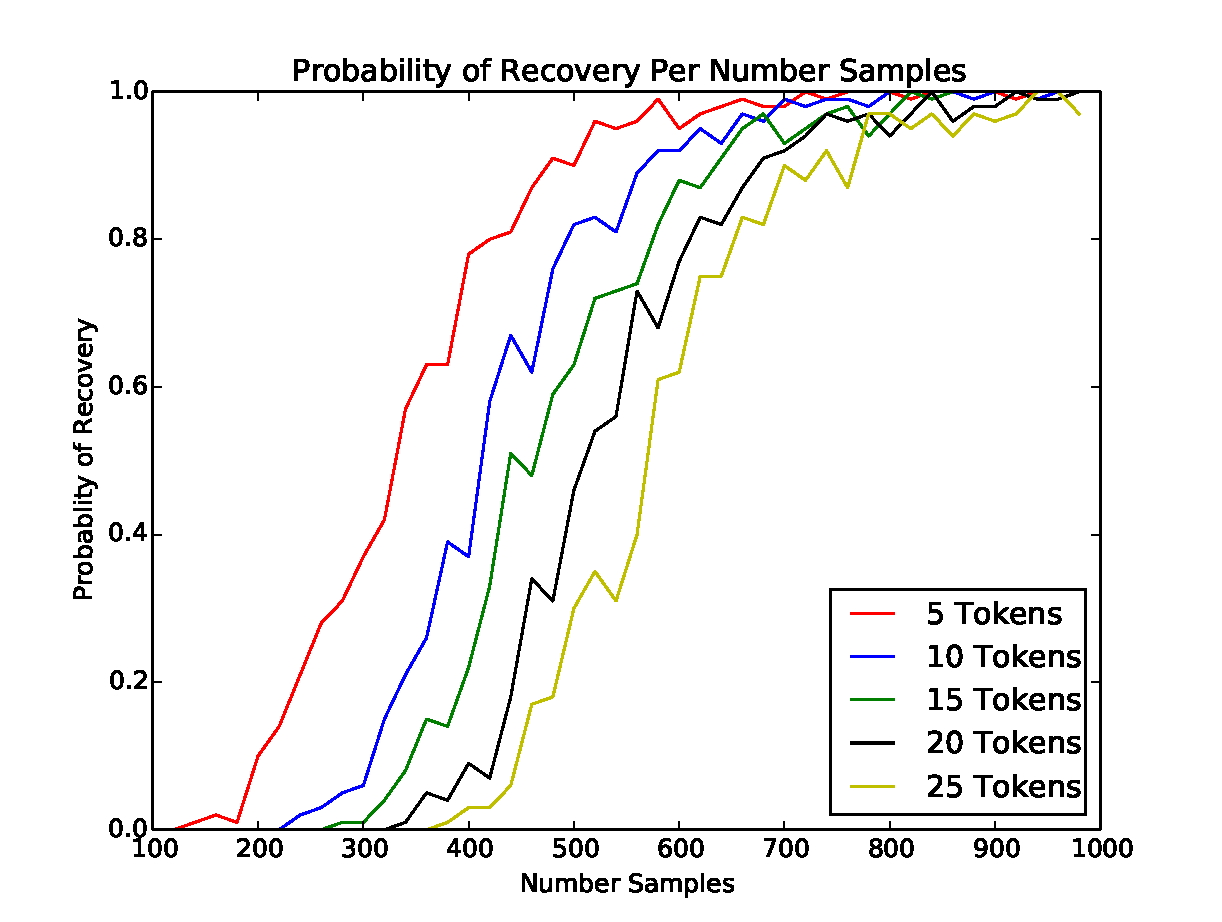
\includegraphics[width=3.5in]{./recovery_probability_per_samples.pdf}
	\caption{Recovery Probability}
	\label{fig:recovery_probability}
\end{figure}
For example, the red curve analyzes a sanitizer that blocks any string containing any one of five distinct patterns. This curve says that the sanitizer can be fully explained with almost 100\% accuracy with about 575 observations. Each observation requires running the sanitizer. This is much better than the alternative of running the sanitizer on a string containing a single pattern, which would require 4970 observations (and 4970 sanitizations)! And with only 300 observations, group testing will correctly identify the malicious patterns 50\% of the time. Since the curves increase rapidly, the additional number of observations to greatly increase the likelihood of success is quite small. This describes the power of group testing. By combining patterns in tests, we can greatly reduce the number of sanitizations required to fully explain the sanitizer, with high likelihood of success.

We now discuss experiments on several of the sanitizers considered above in Section \ref{ss:sanitizers}. Of course, there is a large dependence on $p$ versus the number of samples. Recall that we need to observe enough blocked and unblocked strings in order to learn the sanitizer. We first consider Sanitizer 1 matches a single pattern ``$\sf{</alphanumerictext>}$". With $p=.01$, our framework outputs \textbf{Pattern 4902: $\sf{('</', '>')}$ has value 1.0}, i.e., it easily outputs the correct explanation of Sanitizer 1. And with only 400 samples and a single malicious pattern, there were only two blocked strings to learn from.

But a single malicious pattern is easy to catch as long as $p$ is large enough to observe it in at least one string. We next consider Sanitizer 5 which matches the two patterns ``$\sf{</alphanumerictext>}$" and ``$\sf{(alphanumerictext)}$". Twelve out of the 400 sample strings were blocked, however three patterns were found to explain the sanitizer; the framework output \textbf{Pattern 1136: $\sf{('(', ')')}$ has value 1.0, Pattern 3656: $\sf{('url(', ')')}$ has value 1.0, Pattern 4902: $\sf{('</', '>')}$ has value 1.0}. Even though we use delimiters, note that the pattern $\sf{('url(', ')')}$ contains as a sub-pattern $\sf{('(', ')')}$, so that both patterns are blocked for the same reasons. The framework currently does not differentiate between these patterns. This example shows successful explanation of the sanitizer with only 400 samples, along with one of the current drawbacks. When we similarly consider Sanitizer 7, we learn only two patterns with the framework outputting \textbf{Pattern 1136: $\sf{('(', ')')}$ has value 1.0, Pattern 4902: $\sf{('</', '>')}$}. Now, only nine strings were blocked, however, due to the delimiters included in the sanitizer, the correct explanation was found.
	
We finally consider Sanitizers 4 and 6 with the most malicious patterns. Running our framework on Sanitizer 4 (without delimiters) matches 376/400 random strings.  With so few unblocked strings, it is difficult for group testing to correctly explain the sanitizer, and indeed, the linear program results in an $x$ with 339 nonzero entries, rather than the four that correctly explain the sanitizer. Meanwhile, the same experiment with Sanitizer 6 (with delimiters) correctly explains the sanitizer with the output \textbf{Pattern 1: $\sf{script}$ has value 1.0, Pattern 12: $\sf{javascript:}$ has value 1.0, Pattern 1136: $\sf{('(', ')')}$ has value 1.0, Pattern 4902: $\sf{('</', '>')}$ has value 1.0}. This means that group testing can be a very powerful tool for explaining sanitizers, and extending the tools we currently understand to account for ordering would make group testing even more powerful here.

\section{Related Work}

We divide our discussion of related work into two parts: software testing and compressed sensing.

\subsection{Software Testing} 

The delta-debugging algorithm \cite{DeltaDebugging:2000,DeltaDebugging:2002} generalizes and simplifies a failing test case into a minimal failing test, and also isolates the difference between a failing and a passing test. The underlying idea is to systematically simplify the failing scenario until the root cause of failure is uncovered, and dually, if a passing scenario is also available, then that scenario is evolved into a scenario that is increasingly similar to the failing scenario.

The goal of isolating the cause of failure is conceptually similar to our goal of obtaining a minimal characterization of the target system's behavior. However, from a technical perspective, our approach --- grounded in the theory of group testing --- is quite distinct. The process is not iterative (at least in the offline variant), and there are formal guarantees that govern the complexity of our technique.

The XSS Analyzer system \cite{TrippIssta:2013}, designed to test web applications for XSS vulnerabilities, is guided by an online feedback loop. The key idea is to (i) learn from a failing input $i$ what the reason for the failure was by testing the target system with the tokens $i$ consists of, and (ii) if one or more of these tokens also fail in isolation, prune all inputs that include a failing token.

A key difference between our approach and XSS Analyzer is that XSS Analyzer can only handle single-token-based sanitization, and not regular expressions that range over combinations of tokens. In the latter case, combinatorial explosion would degrade the process into an unscalable testing solution. With our approach, in contrast, the combinatorial complexity is mitigated by drawing correlations between token combinations and failures according to the theory of group testing.

Wang et al. \cite{YH-Wang:2010} also focus on security testing. They propose a learning approach to synthesize effective XSS payloads. Their technique proceeds byfirst mining real-world XSS payloads,
then decomposing each payload into its constituting elements,
and finally building a hidden Markov model of the
connections between the different elements, which permits
synthesis of mutated XSS attacks.

A main difference from our approach is that we focus on a particular software system, in fingerprinting its behavior, whereas Wang et al. generate XSS payloads in an open-world setting. This is of course valuable, but given a specific subject $S$ for testing, our approach (similarly to XSS Analyzer) targets $S$ in particular and so it is more effective.

Closer to our goal of creating a model for a black-box system is the testing solution by Doup\'e et al. \cite{Doupe:2012}. Their goal is to create a state-machine representation of web applications, which captures
how the state of the web application changes as a function of the requests it receives. Doup\'e et al. et al. utilize a heuristic, whereby if the same request was sent twice but different responses were received, then a state change has occurred. Similarly, Amalfitano et al. \cite{Amalfitano:FT08} model, under black-box assumptions, the behavior of rich internet applications (RIAs) as a finite state machine. In this case, the states are the DOM configurations, and the transitions are the UI events that relate between configurations. The analysis interleaves two types of steps: \emph{extraction} (to trace event-driven client configuration and \emph{abstraction} (to cluster together equivalent configurations).

We, too, propose a form of reverse engineering, though we target a different scope and utilize a different technique. As such, we view our contributions in this paper as complementary to these works: We model the system's response to data inputs, while Doup\'e et al. and Amalfitano et al. focus on request and event-driven behaviors, respectively.

For further reading on black-box testing, and security testing in particular, we refer the reader to Bau et al. \cite{Bau:2010} and references therein. For a detailed survey of web-application validation bypass techniques, we point to Offutt et al. \cite{Offutt1,Offutt2,Offutt3}. 

\subsection{Compressed Sensing}

\section{Conclusion and Future Work}

We have presented a promising approach to optimize software testing under black-box assumptions. The key idea is to first create a model of the software system by characterizing its behavior based on random inputs, organized into groups (the key optimization), then selecting one or more tests that appear effective according to the computed model.

An important feature of our approach is the clear formal guarantees that we articulate regarding the complexity of testing (i.e., the number of tests/inputs involved) and the probability of success. We achieve this through use of a technique from the area of signal processing known as compressed sensing, and in particular its Boolean instantiation known as group testing.

In our experiments so far, we have validated the feasibility of group testing as a basis for software testing in the context of integrity assessment. We demonstrated our ability to build an effective model of XSS defenses, including in particular nontrivial regular expressions (beyond the reach of existing state-of-the-art techniques), efficiently and accurately. With our solution, only XXX tests were required on average compared to an average of XXX tests in the case of brute-force testing.

Our two main plans for the future are to extend the scope of our experiments to other testing problems as well as implement an open-source reusable framework for software testing based on compressed sensing. These naturally are related goals, since the hope is that once the framework is available, members of our community will make use of it to enable more clients, and on the other hand, experimenting with multiple clients will guide us in capturing reusable elements and abstractions as part of the framework.

A concrete example of a client that we are interested to implement next is compiler testing. Here individual inputs correspond to different pieces of the language syntax, and the goal is to efficiently isolate specific fragments of the syntax that the compiler doesn't handle correctly. Our experience lately with the Swift compiler suggests that this is a tedious and nontrivial task, and hence, motivates to address it via group testing.

\balance
\bibliographystyle{abbrvnat}
\bibliography{pldi15}



\end{document}

